Finite element method is a classic numerical method for solving partial differential equations. In this chapter, we 
will give a brief introduction to this method. discuss its basic properties and error estimates. In later chapters, we 
will show that the neural network functions can be viewed as an extension of finite element function. 
In this chapter, we discuss the classical linear finite element spaces, the error estimate of the 
finite element method and adaptivity method to improve the
approximation. For shape-regular mesh, we will establish both the upper and lower bound of the 
approximation error. 

%In particular, we will show that the upper convergence 
%rate is also lower bound of the finite element method. This reveals the approximation
%of finite element method is optimal. 

\section{Linear finite element spaces}\label{FEspace}
In this section, we introduce linear finite element spaces. We will walk through the basic setup, 
and derive some error estimates. 
%nodal basis functions and interpolation error estimate of linear finite element spaces. 

\subsection{Triangulations}

%-----------notation introduction--------------------------------------------------------------------

%\subsection{Shape-regular and quai-uniform triangulations}
Given a bounded polyhedral domain $\Om\subset \mathbb {R}^d$, a geometric
triangulation (also called mesh or grid) $\mathcal T_h=\{\tau\}$ of $\Omega$ is a
set of $d$-simplices such that
\begin{enumerate}
\item[(1)] $\overline \Omega=\cup \tau$, where $ \overline \Omega$ denotes the closure of $\Omega$. 
%\item[(2)] for each $\tau\in \mathcal T_h$, $\tau$ is a close set with positive volume. 
\item[(2)]  if $\tau_1$ and $\tau_2$ are distinct elements in $\mathcal T_h$ then $\stackrel{\circ}{\tau _1}\cap \stackrel{\circ}{\tau _2} = \varnothing$, where $\stackrel{\circ}{\tau _i}$ denotes the interior of $\tau_i, i=1,2$ . 
\end{enumerate}
Examples of triangulations for $\Omega=(0,1)$ ($d=1$) and for $\Omega=(0,1)^2$ ($d=2$) are shown in
Figure~\ref{fig:1dpartition} and Figure~\ref{2duniform}, respectively.

\begin{figure}
\setlength{\unitlength}{0.14in} % selecting unit length
\begin{center} % used for centering Figure
\begin{picture}(32,1) % picture environment with the size (dimensions)
\put(8,0){\line(1,0){16}}
\put(8,0){\line(0,1){0.3}}
\put(7.5,1){$x_0$}
\put(9,0){\line(0,1){0.3}}
\put(10,0){\line(0,1){0.3}}
\put(11,0){\line(0,1){0.3}}
\put(12,0){\line(0,1){0.3}}
\put(13,0){\line(0,1){0.3}}
\put(14,0){\line(0,1){0.3}}
\put(15,0){\line(0,1){0.3}}
\put(16,0){\line(0,1){0.3}}
\put(15.5,1){$x_i$}
\put(17,0){\line(0,1){0.3}}
\put(18,0){\line(0,1){0.3}}
\put(19,0){\line(0,1){0.3}}
\put(20,0){\line(0,1){0.3}}
\put(21,0){\line(0,1){0.3}}
\put(22,0){\line(0,1){0.3}}
\put(23,0){\line(0,1){0.3}}
\put(24,0){\line(0,1){0.3}}
\put(23.5,1){$x_{n+1}$}
\end{picture}
\end{center}
\caption{1D uniform grid} % title of the Figure
\label{fig:1dpartition}
\end{figure}
\example Given $\Omega=(0,1)$, we consider the mesh:
\begin{equation}\label{partitionyx}
 0=x_0<x_1<\cdots<x_{n+1}=1, \quad x_i=\frac{i}{n+1},\quad (i=0,\cdots,n+1)
 \end{equation}
which is the 1D uniform grid shown in Figure \ref{fig:1dpartition}.
\begin{figure}
\begin{center}
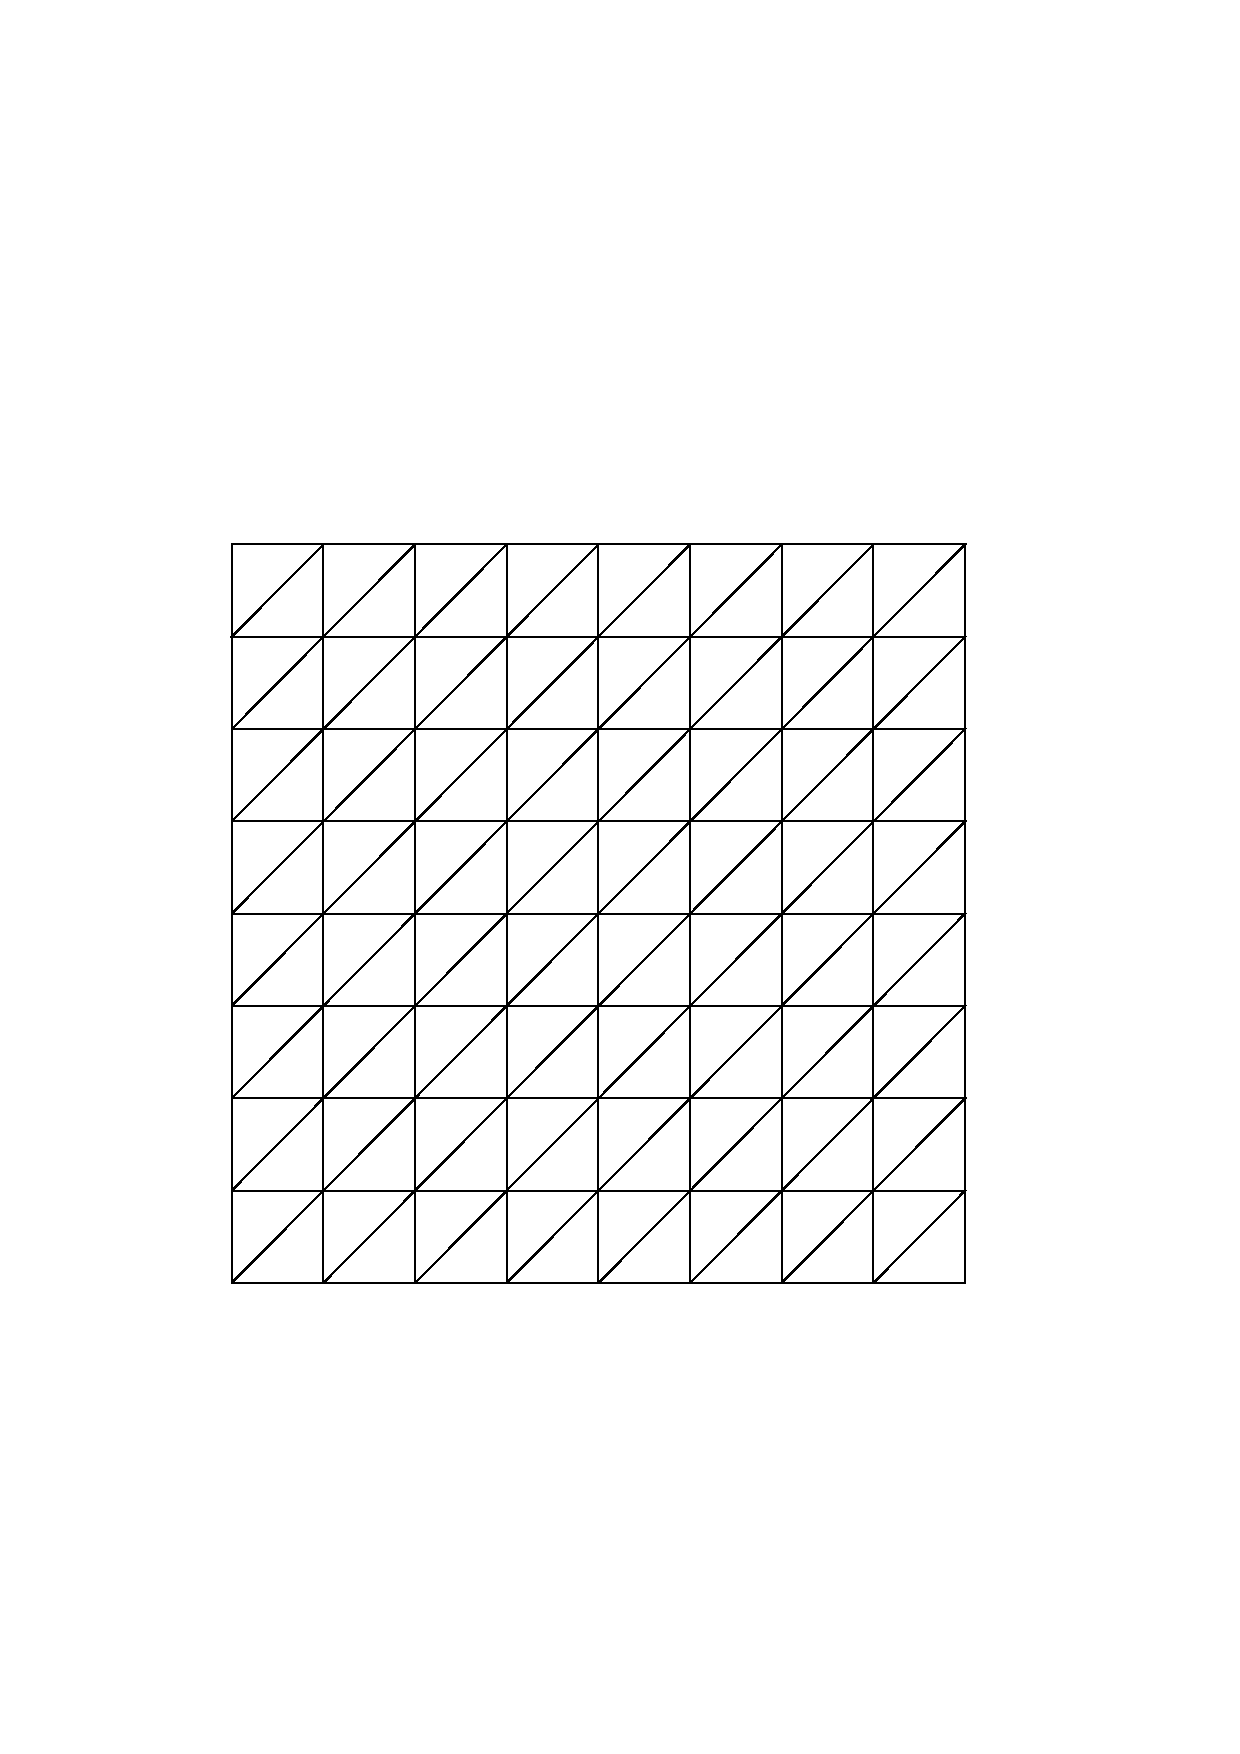
\includegraphics[width=.25\textwidth]{figures/grid1.png} \qquad  \includegraphics[width=.25\textwidth]{figures/u00.pdf}  \qquad \includegraphics[width=.25\textwidth]{figures/2ddiskpartition.pdf}  
\end{center}
\caption{2D grids}
\label{2duniform}
\end{figure}

Denote 
$$
h_\tau=\mbox{\rm diam} (\tau)\quad  \hbox{(diameter of the smallest sphere containing $\overline{\tau}$)},
$$
and 
$$
 h=\max_{\tau\in\mathcal T_h} h_\tau;\quad
\underline{h}=\min_{\tau\in\mathcal T_h} h_\tau.
$$
A set of triangulations $\mathscr T$ is called {\em shape regular} if
there exists a constant $c_0$ such that
\begin{equation}\label{shape} \max _{\tau \in \mathcal T_h} \frac{h_{\tau}^d}{|\tau|}\leq c_0, \quad \forall \, \mathcal T_h\in
\mathscr T,
\end{equation} 
where $|\tau|$ is the measure of $\tau$ in $\mbb R^d$. This assumption can also be represented as
\begin{equation}\Label{A3.1}
\max_{\tau\in\ct_h}\frac{h_\tau}{\rho_\tau}\le\sigma_1,\quad \forall \, \mathcal T_h\in
\mathscr T,
\end{equation}
where $\rho_\tau$\index{$\rho_\tau$} denotes the radius of the ball
inscribed in $\tau$. In two dimensions, it is equivalent
to the minimal angle of each triange is bounded below uniformly
in the shape regular class. 
%We shall define $h_{\tau} = |\tau|^{1/n}$
%for any $\tau \in \mathcal T_h\in \mathscr T$. By (\ref{shape}),
%$h_{\tau}\eqsim {\rm diam}(\tau)$ represents the size of an element
%$\tau \in \mathcal T_h$ for a shape regular triangulation $\mathcal T_h\in
%\mathscr T$.

In addition to (\ref{shape}), if
\begin{equation}\Label{A3.2}
  \frac{\max _{\tau \in \mathcal T_h}|\tau|}{\min _{\tau \in \mathcal T_h}|\tau|} \leq \rho,\quad \forall \, \mathcal T_h\in \mathscr T,
\end{equation}
$\mathscr T$ is called {\em quasi-uniform}. For quasi-uniform grids,
$h=\max _{\tau \in \mathcal T_h} h_{\tau}$, the mesh size of
$\mathcal T_h$, is used to measure the approximation rate. 
%In the FEM literature, we often write as $\mathcal T_h$.

%The triangulation $\thset$ is said to be quasi-uniform
%\index{triangulation, quasi-uniform} if it satisfies \rf{A3.1} and
%the following
%\begin{eqhttps://gmu.zoom.us/j/97581839555?pwd=ZjlZeFE3Q0JkekdOcGpBZEZxdFJwQT09uation}\Label{A3.2}
%h\le\sigma_3 \underline {h}.
%\end{equation}

The assumption \rf{A3.1} is a local assumption, as is meant by above
definition, for $d=2$ for example, it assures that each triangle will
not degenerate into a segment in the limiting case.  
%A triangulation satisfying this assumption is often called to be {\it shape regular}.

On the other hand, the assumption \rf{A3.2} is a global assumption,
which says that the smallest mesh size is not too small compared with
the largest mesh size of the same triangulation.  By the definition, in
a quasi-uniform triangulation, all the elements are about the same size
asymptotically.

Let $ x_{i}=(x^1_{i}, \cdots, x^d_{i})^t, i=1,\cdots, d+1$ be $d+1$ points in $\mbb R^d$ which do not all lie in one hyper-plane. 
The {\it convex hull} of the $d+1$ points $ x_1, \cdots,  x_{d+1}$ (See Figure \ref{fig:barycentricCoor})
\begin{equation}
\tau :=\{ x=\sum _{i=1}^{d+1}\lambda _i x_i \, | \, 0\leq \lambda_i\leq 1, i=1:d+1, \sum _{i=1}^{d+1}\lambda _i=1 \}
\end{equation}
is defined as a {\em geometric $d$-simplex} generated (or spanned) by
the vertices $ x_1, \cdots,  x_{d+1}$. For example, a triangle
is a $2$-simplex and a tetrahedron is a $3$-simplex. For an integer
$0\leq m \leq d-1$, an $m$-dimensional face of $\tau$ is any
$m$-simplex generated by $m+1$ of the vertices of
$\tau$. Zero-dimenisonal faces are vertices and one-dimensional faces
are called edges of $\tau$. The $(d-1)$-face opposite to the vertex
$ x_i$ will be denoted by $F_i$.
\begin{figure}[hpt]
%\subfigure[1d simplex]{
%\begin{minipage}[t]{0.33\linewidth}
\centering
\includegraphics*[width=2.5cm]{figures/barycentricCoor1D.pdf}
%\end{minipage}}%%
%\subfigure[2d simplex]{
%\begin{minipage}[t]{0.33\linewidth}
%\centering
\includegraphics*[width=3cm]{figures/barycentricCoor2D.pdf}
%\end{minipage}}%%
%\subfigure[3d simplex]
%{\begin{minipage}[t]{0.33\linewidth}
%\centering
\includegraphics*[width=3.1cm]{figures/barycentricCoor3D.pdf}
%\end{minipage}}
\caption{Geometric explanation of barycentric coordinates}
\label{fig:barycentricCoor}
\end{figure}
%\paragraph{Barycentric coordinates}
On the other hand, for any $ x\in \tau$, there exist unique numbers $\lambda _1,\cdots, \lambda _{d+1}$ satisfying $\displaystyle 0\leq \lambda_i\leq 1, i=1:d+1, \sum _{i=1}^{d+1}\lambda _i=1$ such that $\displaystyle x=\sum _{i=1}^{d+1}\lambda _i x_i$, thus we can denote $\lambda _1,\cdots, \lambda _{d+1}$ as $\lambda _1( x),\cdots, \lambda _{d+1}( x)$. In fact,  the numbers $\lambda _1( x),\cdots, \lambda _{d+1}( x)$ are
called {\em barycentric coordinates} of $ x$ with respect to the
$d+1$ points $ x_1, \cdots,  x_{d+1}$. There is a simple
geometric meaning of the barycentric coordinates. Given a $ x\in
\tau$, let $\tau _i( x)$ be the simplex with vertices $ x_i$
replaced by $ x$. Then it can be easily shown that
\begin{equation}\label{eq:lambdasolution}
\lambda _i( x) = |\tau _i( x)|/|\tau|,
\end{equation}
where $|\cdot|$ is the Lebesgure measure in $\mbb R^d$, namely area in
two dimensions and volume in three dimensions. Note that $\lambda
_i( x)$ is affine function of $ x$ and vanishes on the face
$F_i$. We list the four basic properties of barycentric coordinate below:
\begin{enumerate}
\item $0\leq \lambda_i( x)\leq 1$;
\item $\displaystyle\sum_{i=1}^{d+1} \lambda_i( x)=1$;
\item $\lambda_i( x)\in P_1(\tau)$, where $P_1(\tau)$ denotes the space of polynomials of degree $1$
(linear) on $\tau\in \mathcal T_h$;
\item $\lambda_i( x_j)=\delta_{ij}=\begin{cases}
1, \quad &\text{if}  \quad  i=j\\
0, \quad &\text{if} \quad i\neq j
\end{cases}.$
\end{enumerate}

\subsection{Continuous linear finite element spaces}\label{linearFE}
A conforming linear finite element function in a domain $\Omega\subset
\mathbb R^d$ is a continuous function that is piecewise linear
function with respect to a grid or mesh consisting of a union of simplices.

Given a shape regular triangulation $\mathcal T_h$ of $\Omega$, we define the 
continuous linear finite element space as 
\begin{equation}\label{LinFE}
V_h:=\{v\,|\, v\in C(\overline \Omega), \,\hbox{ and }\, v|_{\tau}\in
P_1(\tau), \forall \tau \in \mathcal T_h\},
\end{equation}
where $P_1(\tau)$ denotes the space of polynomials of degree $1$
(linear) on $\tau\in \mathcal T_h$. Whenever we need to deal with boundary
conditions, we further define $V_{h,0}=V_h\cap H_0^1(\Omega)$.

We note here that the global continuity is also necessary in the
definition of $V_h$ in the sense that if $u$ has a square interable
gradient, that is $u\in H^1(\Omega)$, and $u$ is piecewise smooth,
then $u$ is continuous. 

We always use $n_h$ to denote the dimension of finite element
spaces. For $V_h$, $n_h$ is the number of vertices of the
triangulation $\mathcal T_h$ and for $V_{h,0}$, $n_h$ is the number of
interior vertices. 

\paragraph{Nodal basis functions and dual basis}
For linear finite element spaces, we have the so
called \emph{a standard nodal basis functions} $\{\varphi
_i,i=1,\cdots n_h\}$ such that $\varphi_i$ is piecewise linear (with
respect to the triangulation) and $\varphi_i(x_j)=\delta_{i,j}$.  Note
that $\varphi _i|_\tau$ is the corresponding barycentrical coordinates
of $x_i$. See Figure \ref{fig:nodalbasis} for an illustration in 2D.
\begin{figure}[hpt]
%\subfigure[1d basis function]{
%\begin{minipage}[t]{0.49\linewidth}
\centering
\includegraphics*[height=4.5cm,width=7cm]{6DL/figures/Dualbasis}
%\end{minipage}}
\caption{Dual basis functions of $V_h$ in 1D for $n_h=5$.}
\label{fig:dualbasis}
\end{figure}
Let $(\varphi_i^*)_{i=1}^{n_h}$ be the dual basis of $(\varphi_i)_{i=1}^{n_h}$, namely
\begin{equation}
  \label{eq:1}
(\varphi_i^*, \varphi_j) =\delta_{i, j}, \quad i, j=1,\ldots, n_h.    
\end{equation}
We notice that all the nodal basis functions $\{\varphi_i\}$ are locally
supported, but their dual basis functions $\{\varphi_i^*\}$ are in general
not locally supported (see Figure \ref{fig:dualbasis}).  The nodal basis functions $\{\varphi_i\}$ are
easily constructed in terms of barycentric coordinate functions.  The
dual basis $\{\varphi_i^*\}$ are only interesting for theoretical
consideration and it is not necessary to know the actual constructions
of these functions.

%
\begin{figure}[hpt]
%\subfigure[1d basis function]{
%\begin{minipage}[t]{0.49\linewidth}
\centering
\includegraphics*[height=4.5cm,width=7cm]{figures/basisfunction}
%\end{minipage}}%%
%\subfigure[2d basis function]{
%\begin{minipage}[t]{0.49\linewidth}
%\centering
\includegraphics[height=5cm,width=7cm]{figures/nodalbasis.pdf}
%\end{minipage}}
\caption{Nodal basis functions in 1d and 2d}
\label{fig:nodalbasis}
\end{figure}
Since $\{\varphi_i,i=1,\cdots n_h\}$ is a basis of $V_h$, therefore for any $v_h\in V_h$, we have the representation
$$
v_h(x)=\sum_{i=1}^{n_h}v_h(x_i)\varphi_i(x). 
$$

Let us see how our construction of continuous linear finite space and the nodal basis looks like  in one spatial dimension. 
Associated with the mesh
$$
\mathcal T_h=\{0=x_0<x_1<\ldots<x_{n_h}<x_{n_h+1}=1\},
$$
by the definition given in \eqref{LinFE} and the definition  $V_{h,0}=V_{h}\cap H_0^1(\Omega)$, we have
\[
\begin{array}{ll}
V_{h,0}=\{v:~\mbox{$v$ is continuous and piecewise linear}~ \mbox{w.~r.~t. $\mathcal T_h$, } v(0)=v(1)=0\}.
\end{array}
\]
A plot of a typical element of $V_{h,0}$ is shown in Fig.~\ref{fig:1dtypical}.

It is easily calculated (as we already mentioned), that the dimension
of $V_{h,0}$ is equal to the number of internal vertices, and the nodal
basis functions spanning $V_{h,0}$ (for $i=1,2,\cdots,n_h$) are (see also
Fig.~\ref{fig:nodalbasis}):
\begin{equation}\label{1dbasis:function}
\varphi_i(x)=\left\{\begin{array}{cl}
\displaystyle \frac{x-x_{i-1}}{h}, & x\in[x_{i-1},x_i];\\
\displaystyle \frac{x_{i+1}-x}{h}, & x\in[x_{i},x_{i+1}];\\
0 &\mbox{elsewhere}.
\end{array}\right.
\end{equation}

\begin{figure}[hpt]
\centering
\includegraphics*[width=2in]{figures/femfunction1.pdf}
\caption{Plot of a typical element from $V_{h,0}$.} 
\label{fig:1dtypical}
\end{figure}



%%%%%%%%%%%%%%%%%%%%END from grid.tex%%%%%%%%%%%%%%%%%%%%%%%%%%%%%%%

%%%%%%%%%%%%%%%%%%%%END from grid.tex%%%%%%%%%%%%%%%%%%%%%%%%%%%%%%%

%%%%%%%%%%%%%%%%%%%%END from grid.tex%%%%%%%%%%%%%%%%%%%%%%%%%%%%%%%
